‌\chapter{‌خواص دنیای محاسبات کوانتومی}
\section{کیوبیت}
کیوبیت‌ها
\LTRfootnote{Qubits}
 در کامپیوترهای کوانتومی، معادل بیت ها
\LTRfootnote{bits}
 در کامپیوترهای کلاسیک هستند. یک بیت یا در حالت صفر قرار دارد یا در حالت یک قرار دارد. تفاوت کیوبیت‌ها در این است که میتوانند حالی به جز صفر یا یک داشته باشند یا میتوان گفت برهم‌نهی 
\LTRfootnote{superposition}
حالات را شاهد هستیم. درنتیجه، کیوبیت میتواند حالات بیشتری از بیت داشته باشد. هر کیوبیت، به یک احتمالی میتواند یک باشد و به یک احتمالی میتواند صفر باشد. 
\begin{equation}
\left|\Psi\right\rangle = \alpha\left|0\right\rangle + \beta\left|1\right\rangle = \begin{bmatrix}
 \alpha
\\
\beta
\end{bmatrix}
\end{equation}
به طوری که 
$\alpha$
 و 
$\beta$
  شدت احتمال هستند و هر دو اعداد مختلط هستند به طوری که
\begin{equation}
\alpha^{2} + \beta^{2} = 1
\end{equation}
فضای حالتی که این دو متغیر تشکیل میدهند، یک فضای مختلط دو بعدی است.  حالات خاص صفر و یک، یک فضای بردار پایه ای
\LTRfootnote{orthonormal basis}
برای این فضای برداری تشکیل میدهند.
\begin{equation}
\left|0\right\rangle = (0, 1) and \left|1\right\rangle = (1, 0)
\end{equation}
در شکل پایین، میتوانید کره بلاچ
\LTRfootnote{Bloch's sphere}
  که نوعی بازنمایی هندسی از حالت یک کیوبیت است، را مشاهده کنید.
\begin{figure}[!h]
\centerline{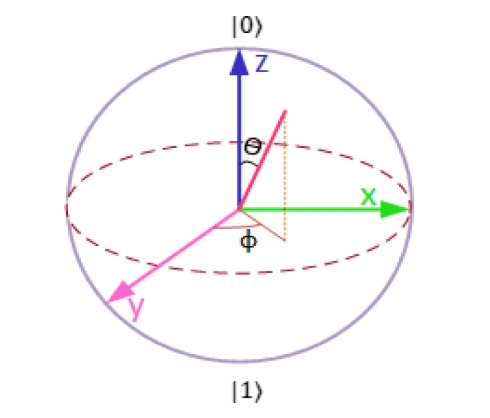
\includegraphics[width=.5\textwidth]{bloch.jpeg}}
\caption{بازنمایی کیوبیت در کره بلاچ}
\end{figure}
این بازنمایی را میتوانید به تعداد نامحدودی کیوبیت هم انطباق دهید. به طوری که با داشتن $n$ کیوبیت نیاز به نگهداری $n^{2}$ عدد خواهید داشت. این حالت زمانی رخ میدهد که $n$ کیوبیت درهم‌تنیده
\LTRfootnote{entangled}
 شوند به طوری که باهم یک حالت را تشکیل دهند و نتوان آنها را جدا کرد. 
\cite{fundamentalsandapplications}
همچنان جمع مجذور همه مقادیر باید برابر با یک شود. نمایش انتزاعی دو کیوبیت به شکل زیر خواهد بود:
\begin{equation}
\left|\Psi\right\rangle = \alpha_{0}\left|00\right\rangle +  \alpha_{1}\left|01\right\rangle +  \alpha_{2}\left|10\right\rangle +  \alpha_{3}\left|11\right\rangle = \begin{bmatrix}
 \alpha_{0}
\\
 \alpha_{1}
\\
 \alpha_{2}
\\
 \alpha_{3}
\end{bmatrix}
\end{equation}
نمایش دو کیوبیت در فرم ماتریسی و دیراک
\LTRfootnote{Dirac}
:
\begin{equation}
\left|00\right\rangle  = \begin{bmatrix}
 \alpha_{1}
\\
 \alpha_{0}
\\
 \alpha_{0}
\\
 \alpha_{0}
\end{bmatrix}
\text{;}
\left|01\right\rangle  = \begin{bmatrix}
 \alpha_{0}
\\
 \alpha_{1}
\\
 \alpha_{0}
\\
 \alpha_{0}
\end{bmatrix}
\text{;}
\left|10\right\rangle  = \begin{bmatrix}
 \alpha_{0}
\\
 \alpha_{0}
\\
 \alpha_{1}
\\
 \alpha_{0}
\end{bmatrix}
\text{;}
\left|11\right\rangle  = \begin{bmatrix}
 \alpha_{0}
\\
 \alpha_{0}
\\
 \alpha_{0}
\\
 \alpha_{1}
\end{bmatrix}
\end{equation}


\section{ضرب تانسوری}
ضرب تانسوری
\LTRfootnote{Tensor product}
، عملیاتی است که بین دو ماتریس میتوان انجام داد. این عملیات، یکی از بخش‌های اصلی محاسبات کوانتومی است. برای اینکه بتوان سیستم‌های چند-کیوبیتی
\LTRfootnote{multiple-qubit systems}
را به صورت ریاضی نمایش داد، از این عملیات استفاده میشود. به این صورت که اگر $M$ یک ماتریس $(p,q)$ باشد و  $N$ یک ماتریس $(x,y)$ باشد، ماتریس ضرب تانسوری آنها یک ماتریس $(px,qy)$ خواهد بود. 
\cite{fundamentalsandapplications}
این ضرب را میتوان با یک گیت کوانتومی
\LTRfootnote{quantum gate}
 اعمال کرد.
\begin{equation}
M =  \begin{bmatrix}
 a_{11} &  a_{12}
\\
 a_{21} & a_{22}
\end{bmatrix}
\text{;}
N =  \begin{bmatrix}
 b_{11} &  b_{12}
\\
 b_{21} &  b_{22}
\end{bmatrix}
\end{equation}

\begin{equation}
M \otimes  N =  \begin{bmatrix}
 a_{11}b_{11} &  a_{11}b_{12} &  a_{12}b_{11} &  a_{12}b_{12}
\\
 a_{11}b_{21} &  a_{11}b_{22} &  a_{12}b_{21} &  a_{12}b_{22}
\\
 a_{21}b_{11} &  a_{21}b_{12} &  a_{22}b_{11} &  a_{22}b_{12}
\\
 a_{21}b_{21} &  a_{21}b_{22} &  a_{22}b_{21} &  a_{22}b_{22}
\end{bmatrix}
\end{equation}
برای ضرب تانسوری دو کیوبیت خواهیم داشت:
\begin{equation}
\left|0\right\rangle  \otimes  \left|1\right\rangle  =
\begin{bmatrix}
1 \\ 0 
\end{bmatrix} 
\otimes
\begin{bmatrix}
0 \\ 1 
\end{bmatrix} 
=
  \begin{bmatrix}
0
\\
1
\\
0
\\
0
\end{bmatrix} = \left|01\right\rangle
\end{equation}

\section{اصل برهم‌نهی}
در دنیای روزمره، همه اشیا، حتی زمانی که به آنها نگاه نمیکنیم، در یک حالت مشخص قرار دارند. این موضوع برای اجسام کوچک همانند کیوبیت ها صدق نمیکند. یک جسم بسیار کوچک میتواند در یک زمان، در چند مکان باشد. در نتیجه، به جای اینکه بگوییم جسم در یک جا قرار دارد، میگوییم در برهم‌نهی قرار دارد. نه تنها مکانش میتواند در چند حالت باشد، بلکه سطح انرژی، شتاب، و خواص کوانتومی آن نظیر چرخش
\LTRfootnote{spin}
 میتواند در چند حالت باشد. 
\\
ما نمیتوانیم این برهم‌نهی را مشاهده کنیم. به محض مشاهده کیوبیت، یا در واقع اندازه گیری آن، حالت آن به یک حالت واحد تبدیل میشود و همه ی مقادیرش ثابت میشوند. در نتیجه، یکی از چالش‌های محاسبات کوانتومی، مشاهده نکردن کیوبیت‌ها در طول فرآیند است. کیوبیت‌ها تنها در آخرین مرحله ی الگوریتم باید مشاهده شوند.
\cite{cambridgebook}
\section{اصل درهم‌تنیدگی}
کیوبیت‌ها خاصیت درهم‌تنیدگی
\LTRfootnote{entanglement}
دارند. به این صورت که با اندازه‌گیری برخی از آنها، مقدار برخی دیگر مشخص میشود و آنها هم مشاهده میشوند. این حالت به فاصله دو کیوبیت ربطی ندارد. درنتیجه میتوان دو کیوبیت را در هم تنید و از هم تا بینهایت دور کرد. سپس، اگر یکی از آنها مشاهده شود، حالت دیگری هم مشخص میشود و به یک حالت واحد تبدیل میشود. این حالت درهم‌تنیدگی همچنان باقی خواهند ماند. نمایش ریاضی درهم‌تنیدگی زمانی است که نتوان حالت شامل چند کیوبیت را به ضرب تانسوری آن کیوبیت‌ها تبدیل کرد. در واقع ضربی وجود نخواهد داشت که آن حالت نهایی را درست کند. درهم‌تنیدگی را میتوان با استفاده از گیت‌های کوانتومی انجام داد. درهم‌تنیدگی در حوزه رمزنگاری و انتقال داده استفاده بخصوص دارد.
\cite{cambridgebook}
\section{برگشت‌پذیری و گیت‌های کوانتومی}
محاسبات کوانتومی وابستگی حیاتی به محاسبات برگشت‌پذیر
\LTRfootnote{reversible calculation}
 دارد. برگشت‌پذیری یعنی بتوان ورودی را با توجه به دانستن خروجی و تابع، بدست‌آورد. برای مثال در کامپیوتر کلاسیک گیت‌ $NAND$ برگشت‌ناپذیر و گیت $NOT$ برگشت‌پذیر است. در نتیجه این خاصیت، هیچ داده و انرژی‌ای از بین نمیرود.
\\
همه گیت‌های کوانتومی باید خاصیت برگشت‌پذیری را داشته باشند. این برتری محاسبات کوامتومی به محاسبات کلاسیک است. گیت‌های کوانتومی بر روی مقدار کوچکی از کیوبیت ها عملیات انجام می‌دهند و بلوک‌های ساخت مدارهای کوانتومی هستند. گیت‌های پایه و لازم کوانتومی شامل $H, X, Y, Z, T, I$ و گیت فاز
\LTRfootnote{phase gate}
میباشد. همچنین گیت‌های $NOR, OR, AND, XOR$ را نیز میتوان پیاده‌سازی کرد. گیت هایی که ورودی $n$ کیوبیت دارند، با یک ماتریس $2^{n} * 2^{n}$ نمایش داده میشوند.
\cite{fundamentalsandapplications}
\begin{figure}[!h]
\centerline{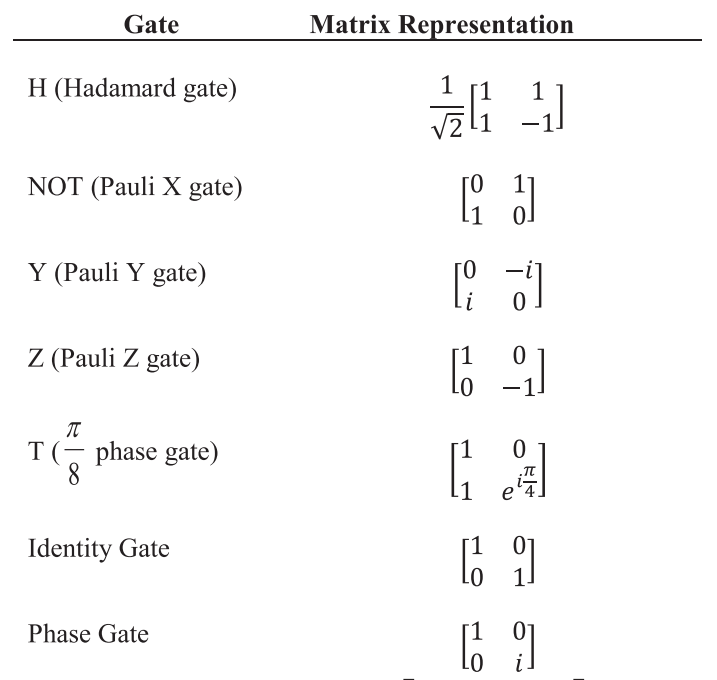
\includegraphics[width=.7\textwidth]{gates.png}}
\caption{بازنمایی ماتریسی برخی از گیت‌های کوانتومی}
\end{figure}